%% ------------------------------------------------------------------------- %%
\chapter{Visão geral}
\label{cap:visao-geral}

\section{Descrição}

Sejam $a$ e $b$ dois vértices de uma árvore enraizada. Define-se como \LCA\ entre eles o vértice mais profundo que contém ambos $a$ e $b$ em sua subárvore. Para ilustrar melhor o problema, uma árvore simples é apresentada na figura~\ref{fig:grafo-simples}.

\begin{figure}[htb]
\begin{center}
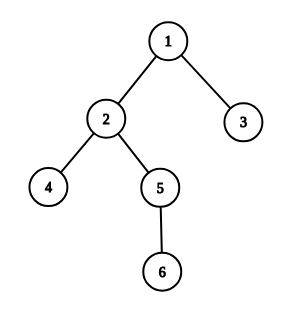
\includegraphics[width=7cm]{images/graph}
\end{center}
\caption{\label{fig:grafo-simples}Árvore simples.}
\end{figure}

A partir desta árvore, podemos notar que o vértice 2 é o \LCA\ entre 4 e 6. Afinal, os únicos dois candidatos ao \LCA\ destes nós são 1 e 2, já que estes são os dois vértices que contêm tanto 4 quanto 6 em suas subárvores. Entretanto, da definição vem que o \LCA\ é sempre o vértice com maior profundidade na árvore, e neste caso é o 2 (vértice 1 possui profundidade 1, vértice 2 possui profundidade 2).

Um caso que merece destaque é o \LCA\ entre 1 e 3, que é 1. Note que pode ocorrer do \LCA\ entre dois vértices ser um deles.

\vspace{50px}

\section{Unicidade}

\begin{definition}
\label{unicidade}
Em uma árvore enraizada, o \LCA\ entre dois vértices é sempre único.
\end{definition}

\noindent
\textbf{Prova: }
Suponha por absurdo que existam dois vértices $x$ e $y$ que sejam simultaneamente \LCA\ de dois vértices $a$ e $b$. Da definição de \LCA\ deve valer que a profundidade de $x$ seja igual à profundidade de $y$. Logo, existem dois caminhos diferentes para chegar na raiz partindo de $a$: um que passa por $x$, e outro que passa por $y$ (de forma análoga o mesmo vale para os caminhos que partem de $b$). Conclui-se que chegamos em uma contradição, pois em uma árvore existe apenas um único caminho da raiz até cada vértice. Portanto, o \LCA\ entre dois vértices em uma árvore é sempre único. A figura~\ref{fig:grafo-nao-arvore} ilustra um possível grafo com esse cenário.

\begin{figure}[htb]
\begin{center}
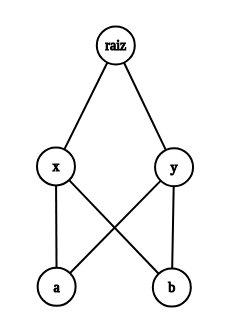
\includegraphics[width=5cm]{images/graph2}
\end{center}
\caption{\label{fig:grafo-nao-arvore}Grafo gerado através da suposição absurda.}
\end{figure}



\section{Algoritmo simples}

Agora que sabemos que para todo par de vértices em uma árvore enraizada sempre existe um único \LCA\, vamos introduzir um algoritmo simples inicial para calculá-lo.

Inicialmente, usaremos um mapa (chave, valor) para guardar a profundidade de cada vértice em relação à raiz. Para preencher este mapa, basta executar uma busca em profundidade (\emph{DFS - Depth First Search}) a partir da raiz.


\begin{algorithm}[H]
\caption{Cálculo da profundidade de cada vértice usando uma \emph{DFS}}
\begin{algorithmic}[1]
\Function{\textsc{CalculaProfundidade}}{vertice,\ nivel}
    \State $profundidade[vertice] \rec nivel$
    \For{cada $filho$ em $filhos[vertice]$}
        \State $CalculaProfundidade(filho,\ nivel+1,\ profundidade)$
    \EndFor
\EndFunction
\end{algorithmic}
\end{algorithm}


Deve-se inicializar $profundidade$ com zeros (vamos usar este valor como um indicador de que a profundidade de um vértice ainda não foi calculada) e chamar a função com os argumentos $(raiz, 1, profundidade)$.

A complexidade de tempo de uma busca em profundidade é $O(n+m)$, onde $n$ é a quantidade de vértices e $m$ a quantidade de arestas. A complexidade de espaço é $O(n)$.

Agora, considere o seguinte algoritmo que encontra o \LCA\ entre dois vértices $a$ e $b$:


\begin{algorithm}[H]
\caption{Determina o \LCA\ entre dois vértices}
\begin{algorithmic}[1]
\Function{\textsc{LCA\_Simples}}{a,\ b}
    \If {$profundidade[a] < profundidade[b]$}
        \State troca($a$, $b$)
    \EndIf
    \While { $profundidade[a] > profundidade[b]$}
        \State $a \rec pai[a]$
    \EndWhile
    \While { $a$ != $b$}
        \State $a \rec pai[a]$
        \State $b \rec pai[b]$
    \EndWhile
    \\\hspace{5mm} \Return $a$
\EndFunction
\end{algorithmic}
\end{algorithm}


\subsection{Corretude}

Nosso algoritmo parte do pressuposto de que $a$ e $b$ estão na mesma árvore.

O código fixa o vértice $a$ para ser mais (ou pelo menos igualmente) profundo do que $b$ (linhas 2 e 3). A partir disto, sabemos que ao sair do primeiro laço teremos que o vértice atualizado $a$ tem profundidade igual a de $b$. Afinal, no início de cada iteração sempre vale que $profundidade[a] - profundidade[b] \geq 0$. Além disso, $profundidade[b]$ não é alterada enquanto $profundidade[a]$ sempre decresce em 1. Assim, quando a execução do laço é interrompida temos que $profundidade[a] - profundidade[b] = 0$, o que implica que  $profundidade[a] = profundidade[b]$.

A última etapa do algoritmo parte do princípio de que, como $a$ e $b$ estão na mesma árvore e possuem mesma profundidade, os caminhos para seus pais os levam até a raiz simultaneamente. Assim, o último laço é interrompido quando $a = b$, que pela definição é o \LCA\ entre eles por ter sido o primeiro vértice que está tanto no caminho de $a$ quanto de $b$ para a raiz.


\subsection{Complexidade}

Para analisar a complexidade de tempo do nosso algoritmo, vamos verificar quantas operações cada etapa do código executa no pior caso:

\begin{itemize}
    \item \textbf{Linhas 2 e 3}: uma operação cada.
    \item \textbf{Primeiro laço}: sua condição de execução é $profundidade[a] - profundidade[b] > 0$. Para maximizar o valor desta função, é claro que $profundidade[a]$ deve assumir o maior valor possível enquanto $profundidade[b]$ deve assumir o menor. Se a árvore possui $n$ vértices, podemos ter um vértice cuja profundidade é $n$ (a folha da árvore) e outro que tenha profundidade $1$ (raiz). Assim, este laço é executado $n$ vezes no pior caso.
    \item \textbf{Segundo laço}: em um pior caso onde ambos $a$ e $b$ são folhas de uma árvore de $n$ vértices, temos que este laço executará $n$ operações para que os caminhos até a raiz sejam percorridos.
\end{itemize}

Assim, a complexidade de tempo do algoritmo 3 é $O(n)$, onde $n$ é o número de vértices na árvore. Como não utilizamos memória adicional nesta etapa, a complexidade de memória é constante - ou seja - $O(1)$.